\subsection{Definition}
\begin{frame}
  \frametitle{Definition}
  \begin{block}{Zweck}
  	Darstellung einer auf die Elemente einer Objektstruktur anzuwendenden Operation. Das
Design Pattern Visitor ermöglicht die Definition einer neuen Operation, ohne die Klasse der
von ihr bearbeiteten Elemente zu verändern.%
  \end{block}
  
\end{frame}

\subsection{Klassendiagramm - Visitor Pattern}
\begin{frame}
	\frametitle{Observer Pattern}		
	\begin{itemize}
		\item Elemente der Objektstruktur fest
		\item Operationen auf Objektstruktur sollen austauschbar und erweiterbar sein
	\end{itemize}	
  	\begin{figure}
		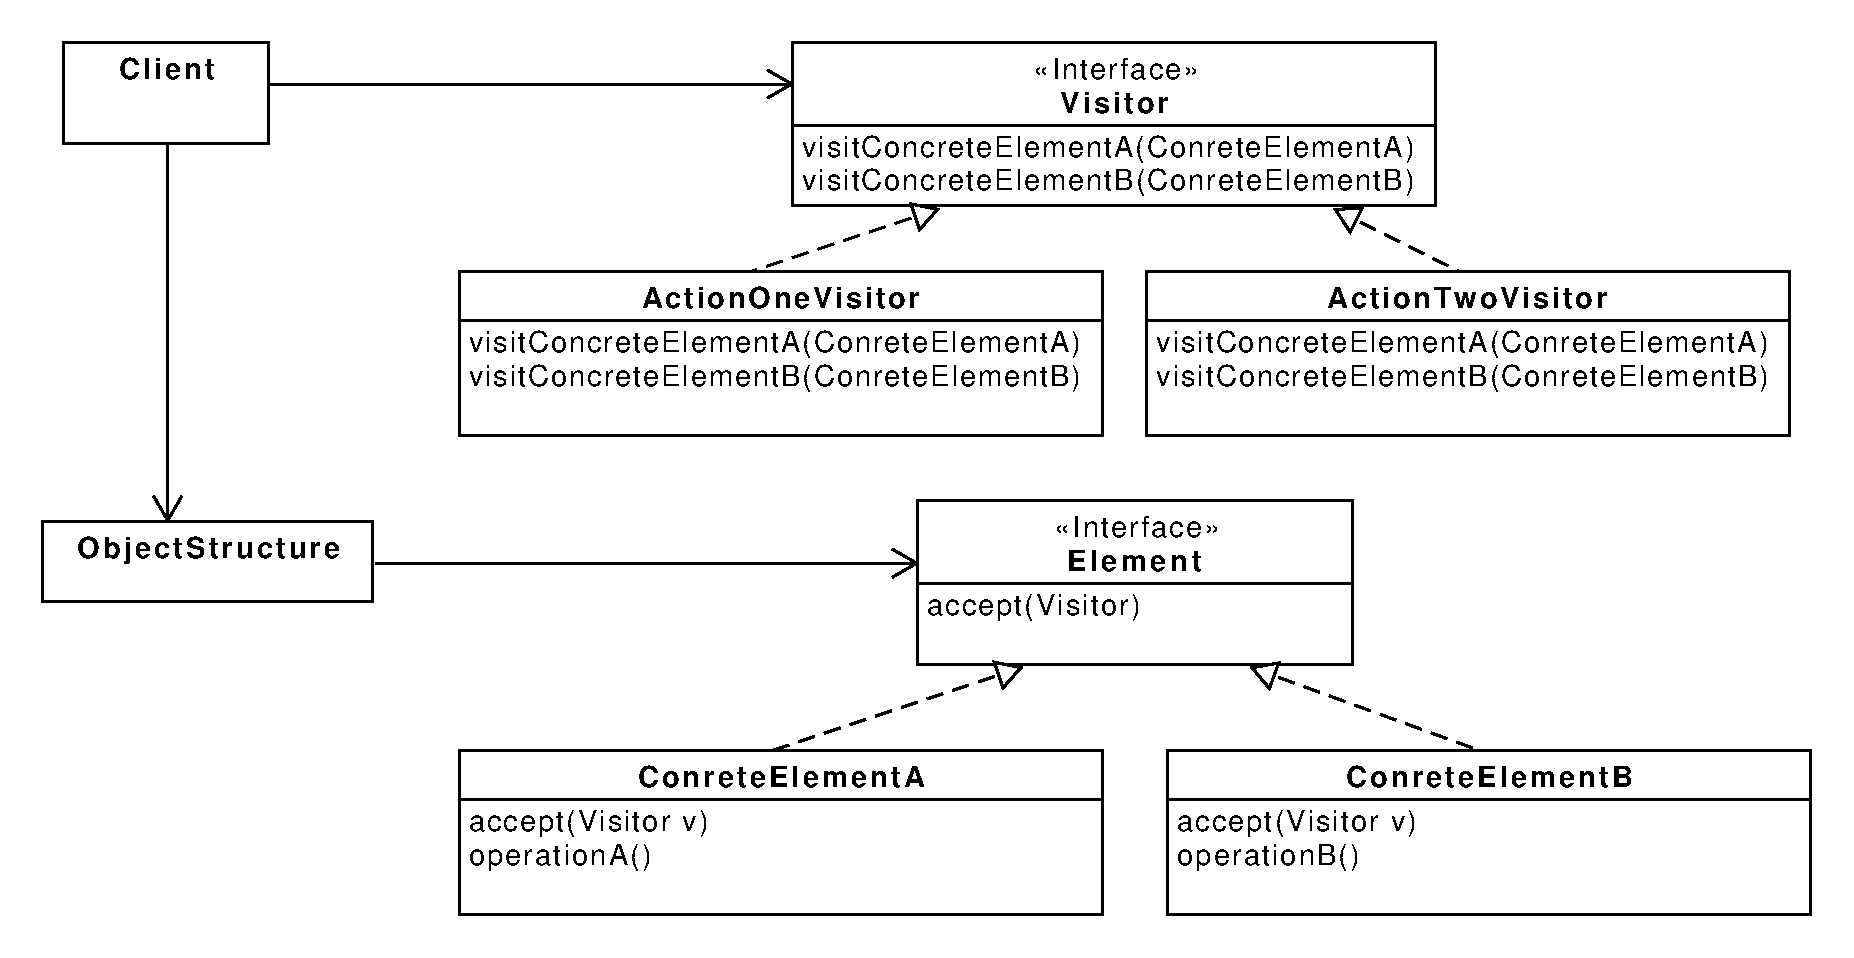
\includegraphics[scale=.3]{paper/visitor/visitor}
	\end{figure}
\end{frame}

\subsection{Beispiel - Kitchen}
\begin{frame}
	\frametitle{Klassendiagramm}
	\begin{itemize}
		\item Die verschiedenen Sorten die wir bearbeiten möchten, bleiben konstant
		\item Wie wir allerdings diese bearbeiten ist noch unklar.
	\end{itemize}	
	
  	\begin{figure}
		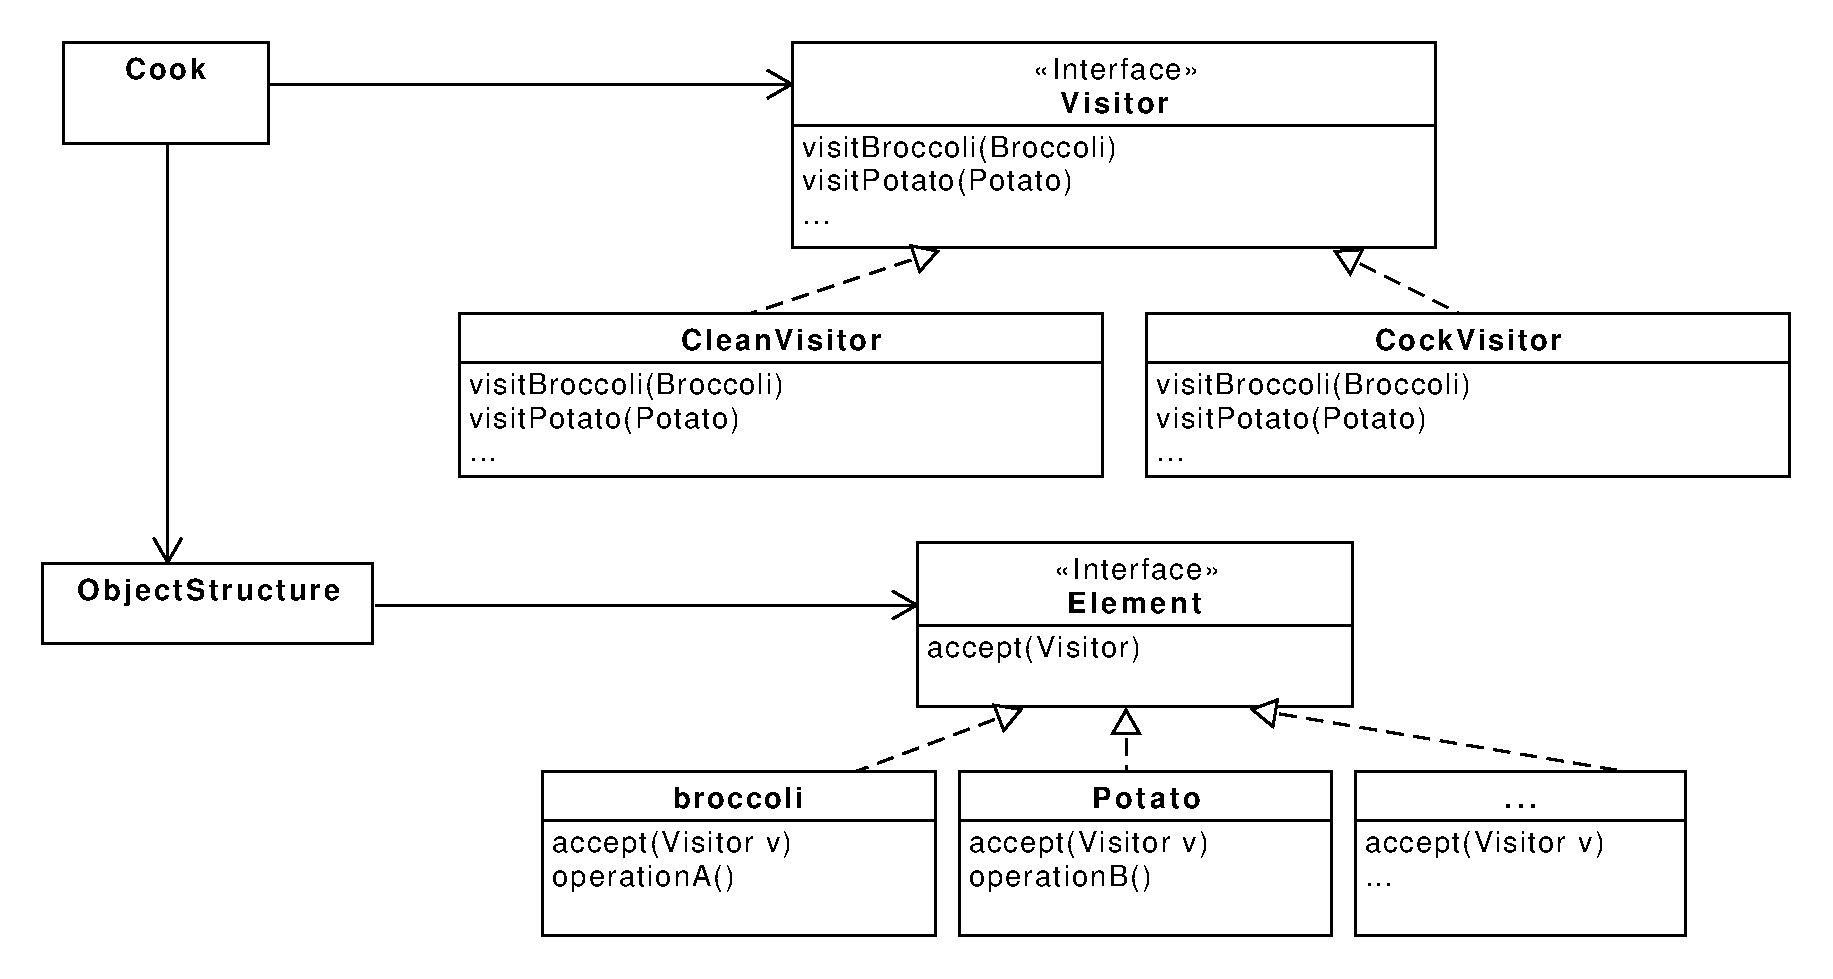
\includegraphics[scale=.3]{paper/visitor/kitchen}
	\end{figure}
\end{frame}



\begin{frame}
	\frametitle{Interfaces}
  	\begin{figure}
		\javacode{resources/visitor_element_interface.java} 
		\javacode{resources/visitor_visitor_interface.java}
	\end{figure}
\end{frame}

\begin{frame}
	\frametitle{Implementierung}
  	\begin{figure}
		\javacode{resources/visitor_potato.java} 
		\javacode{resources/visitor_cleanvisitor.java}
	\end{figure}
\end{frame}

\begin{frame}
	\frametitle{Client}
  	\begin{figure}
		\javacode{resources/visitor_main.java} 
	\end{figure}
\end{frame}

\begin{frame}
	\frametitle{Implementierung}
  \begin{block}{Wer ist für die Traversierung der Objektstruktur verantwortlich}
  	\begin{itemize}
  		\item In der Objektstuktur
  		\item Im Visitor-Objekt
  		\item In einem eigenen Iterator-Objekt
  	\end{itemize}
  \end{block}
\end{frame}


\begin{frame}
	\frametitle{Implementierung}
  \begin{block}{Objektstruktur}
  	\begin{itemize}
  		\item Objektstruktur kümmert sich um die Traversierung 
  		\item Visitor muss der Objektstruktur übergeben werden
  		\item Realisierbar durch z.B Composide-Pattern
  	\end{itemize}
  \end{block}
  \javacode{resources/visitor_composide_example.java} 
\end{frame}

\begin{frame}
	\frametitle{Implementierung}
  \begin{block}{Iterator}
  	\begin{itemize}
  		\item Zugriff auf Elementen einer Objektstruktur, ohne die  Objektstruktur zu kennen.
  		\item Die Visitor-Objekten den Iterator übergeben
  		\item Beim Zugriff eines Elements die accept-Methode aufrufen

  	\end{itemize}
  \end{block}
	\begin{block}{Im Visitor-Objekt}
  	\begin{itemize}
  		\item Objektstruktur wird den konkreten Visitors übergeben
  		\item Visitor übernimmt jetzt die Traversierung
  		\item Nachteil: Traversierung in jedem Visitor
  		\item Vorteil: Flexibler in der Steuerung für bestimmte Aufgaben

  	\end{itemize}
  \end{block}
\end{frame}


\begin{frame}
	\frametitle{Implementierung}

  \javacode{resources/visitor_trav_visitor_object.java} 
\end{frame}